
\documentclass[14pt]{beamer}
\usepackage{graphicx}
\usepackage{fontspec}
\setsansfont{Minion Pro}


\usetheme{UofA}
\newcommand*\chem[1]{\ensuremath{\mathrm{#1}}}
\newcommand*\figcite[1]{\vspace*{\fill}\raggedleft\footnotesize{#1}}

\title[Condensate Cloud]{Mentoring Committee Meeting}
\author{Yifan Zhou}
\institute[UofA]{Steward Observatory\\
University of Arizona}
\begin{document}

{\setbeamertemplate{footline}{}
  \setbeamertemplate{background canvas}[vertical
  shading][bottom=UA_BLUE!15,top=white!20]
  \setbeamertemplate{background}{  \vbox to \paperheight{\vfil\hbox to
      \paperwidth{\hfil
\includegraphics[width=1.5in]{ua_triangle_blue_low}\hfil}}%
    }

\begin{frame}
\maketitle
\end{frame}}

\begin{frame}
  \frametitle{Summary}
  \begin{itemize}
  \item Time resolved HST/WFC3 2-band observation of two low mass
    companions
  \item Looking for variability and studying the vertical structure of
    their atmospheres
  \item A methodology exploration of variability observation in high
    contrast circumstances
  \end{itemize}
\end{frame}

\begin{frame}
  \frametitle{Uniqueness of Low T Atmosphere}
\begin{itemize}
\item Complex chemistry and molecules
\item {Condensation and cloud formation}\\
 Condensate species:\\
 \chem{MgSi_{3}},  \chem{Mg_{2}Si_{4}}, ...\\
to \chem{H_{2}O}, \chem{NH_{3}},...
\end{itemize}
\end{frame}

\begin{frame}
  \frametitle{Clouds at low surface gravity}
  \centering
  \only<1>{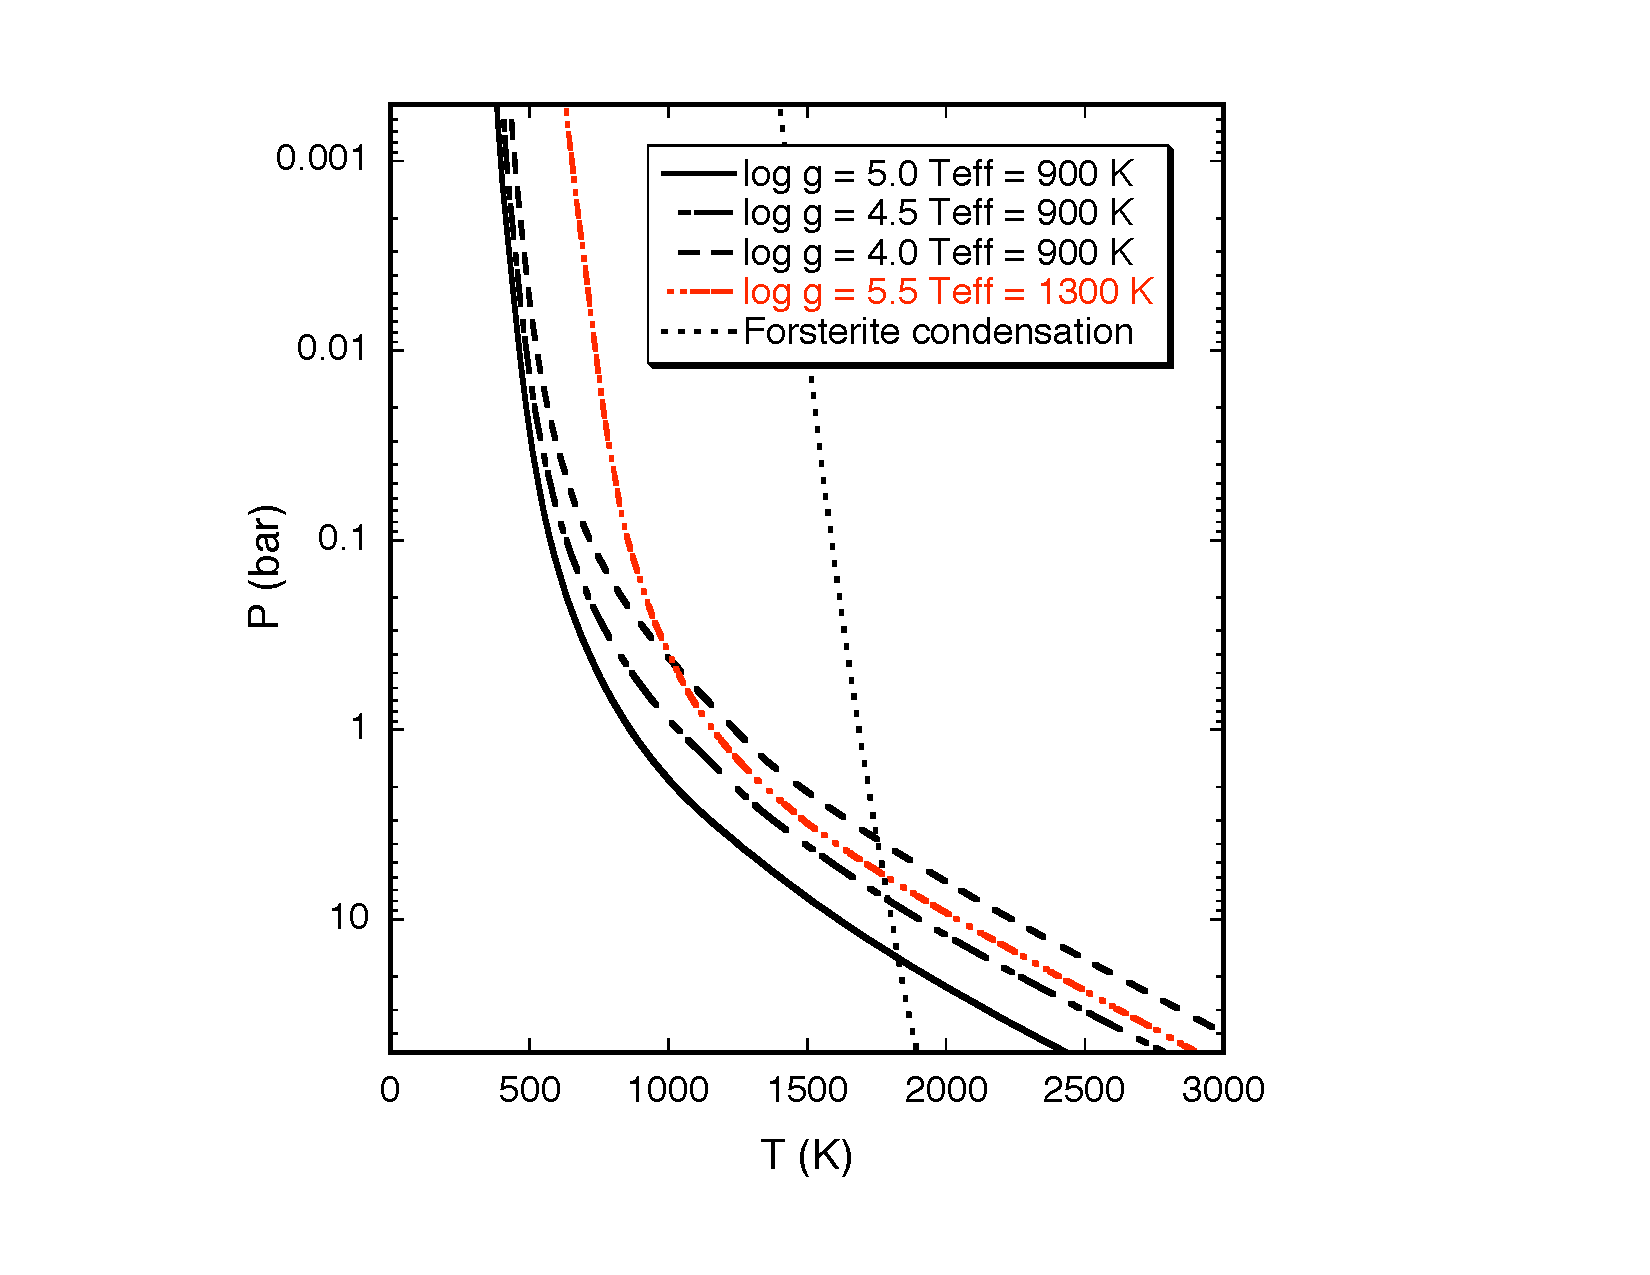
\includegraphics[height=0.8\textheight]{cloud}\\
    \figcite{Marley et al. (2012)}}
  \only<2>{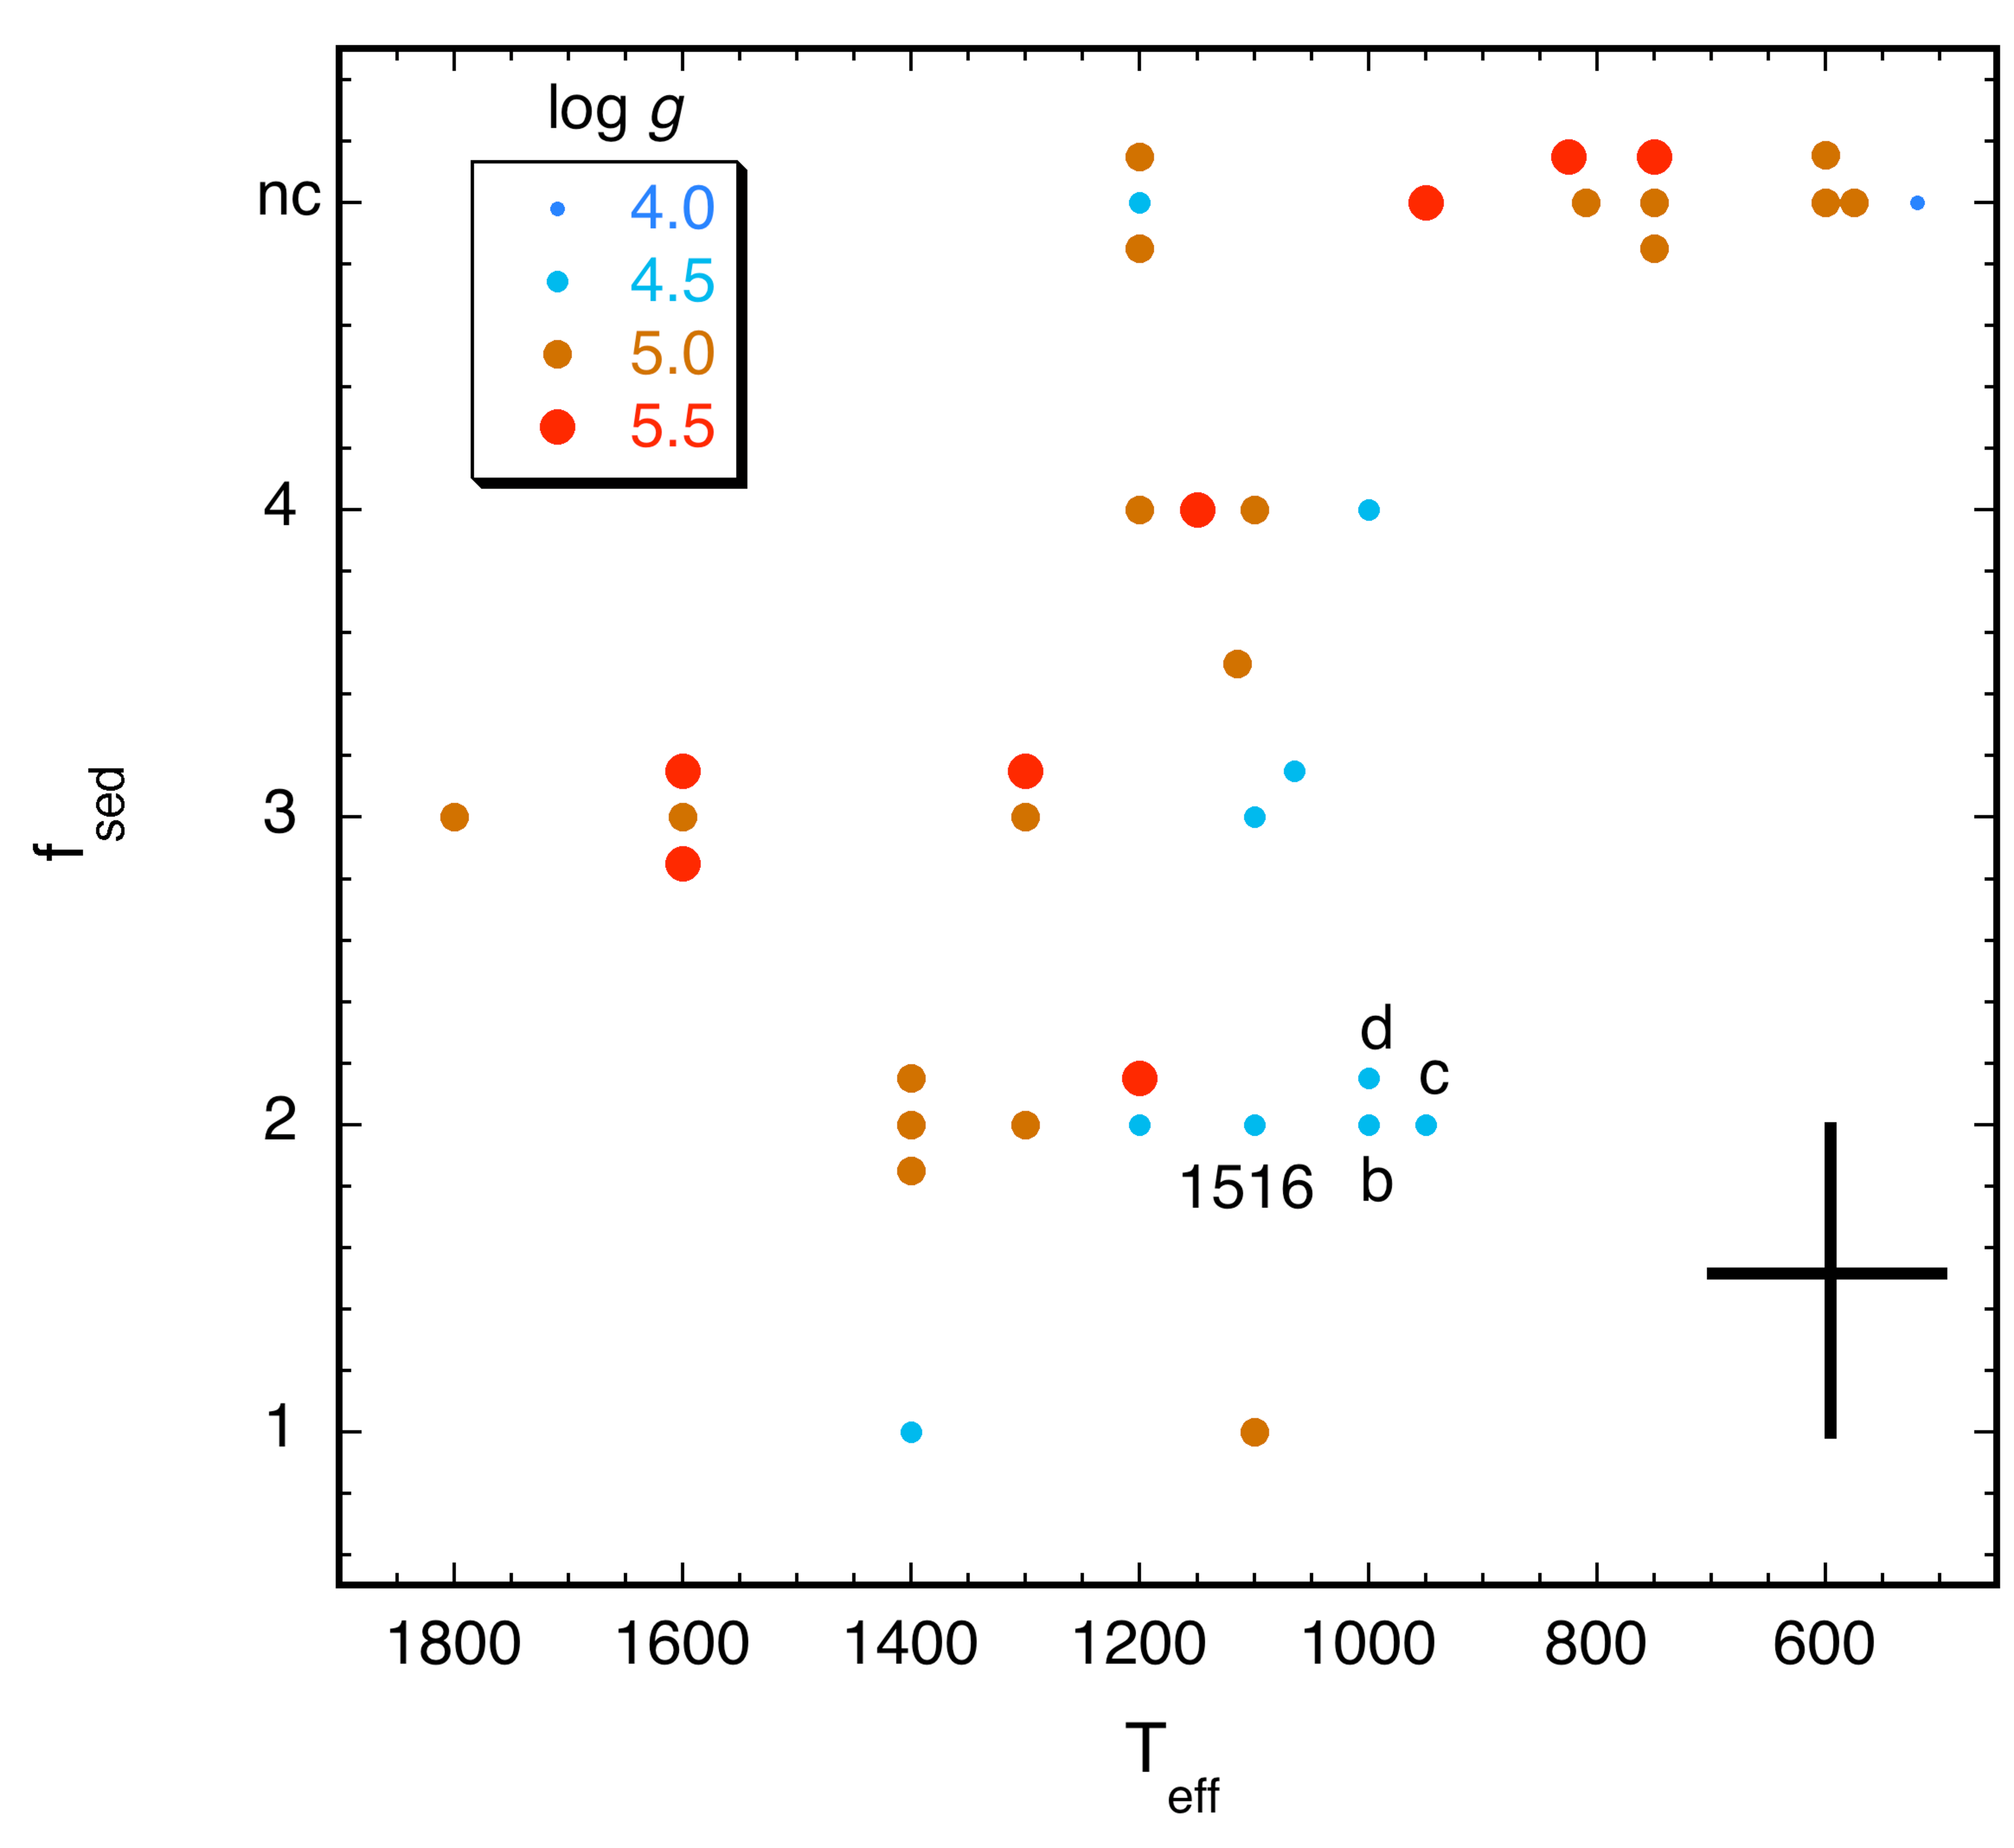
\includegraphics[height=0.8\textheight]{fedvTvsloggs}\\
    \figcite{Marley et. al. (2012)}}
  \only<3>{
    \begin{itemize}
    \item low gravity -> \\
      higher cloud base, larger particle size, thicker clouds
    \item thicker clouds ->? more homogeneous cloud coverage      
    \end{itemize}
}
\end{frame}

\begin{frame}
  \frametitle{Variability of brown dwarfs}
  \centering
  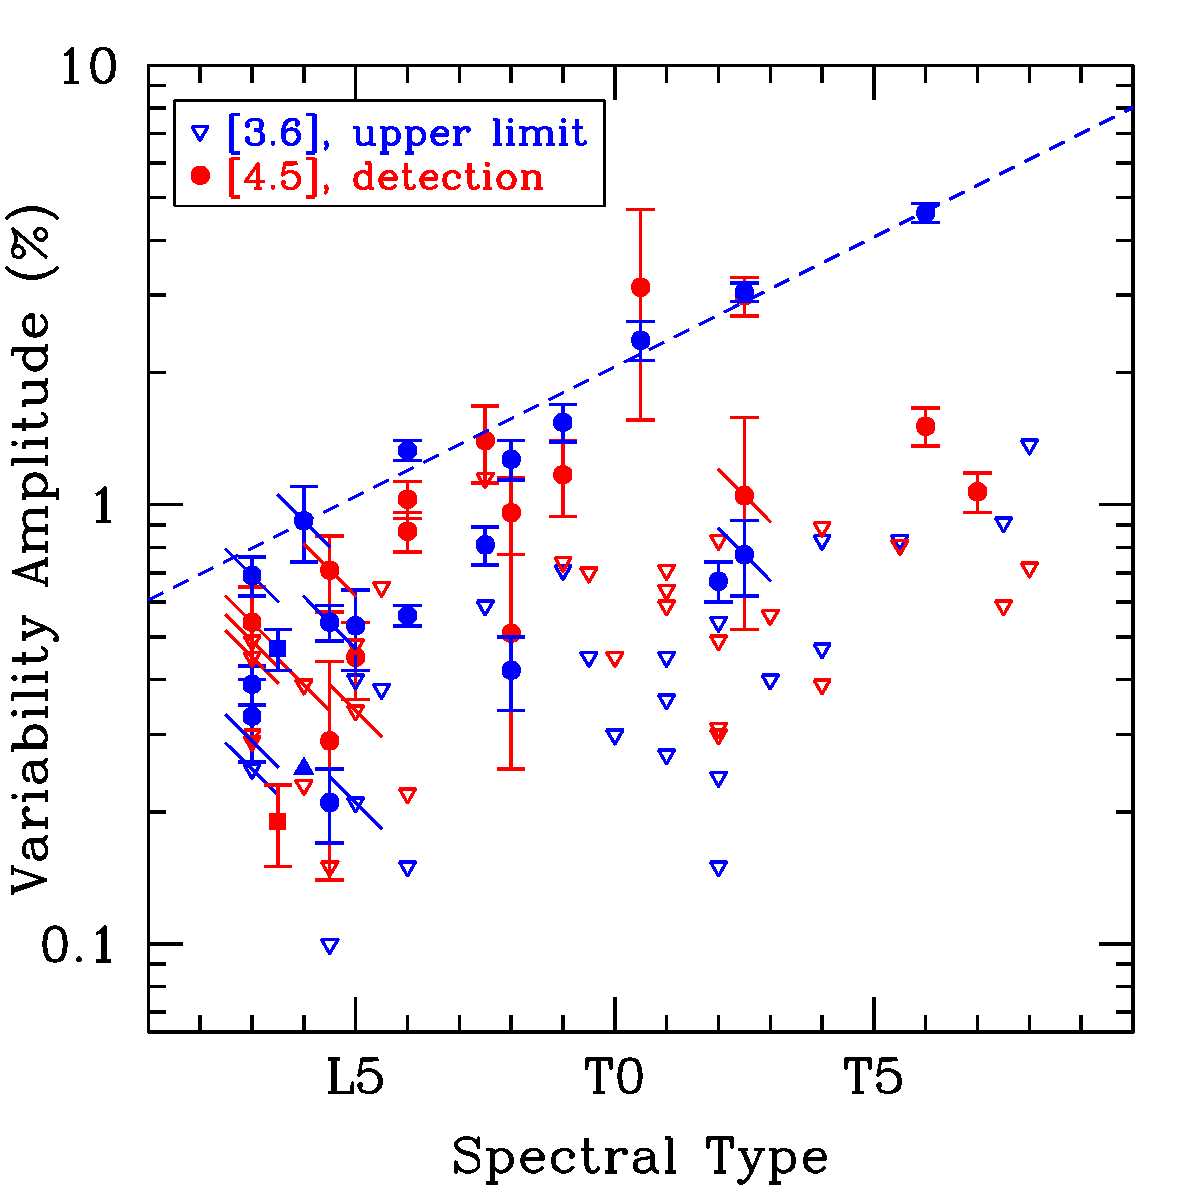
\includegraphics[height=0.8\textheight]{bdVariability}\\
  \figcite{Metchev et. al. (2015)}
\end{frame}

\begin{frame}
  \frametitle{Reducing Scattering}
  \centering
  \only<1>{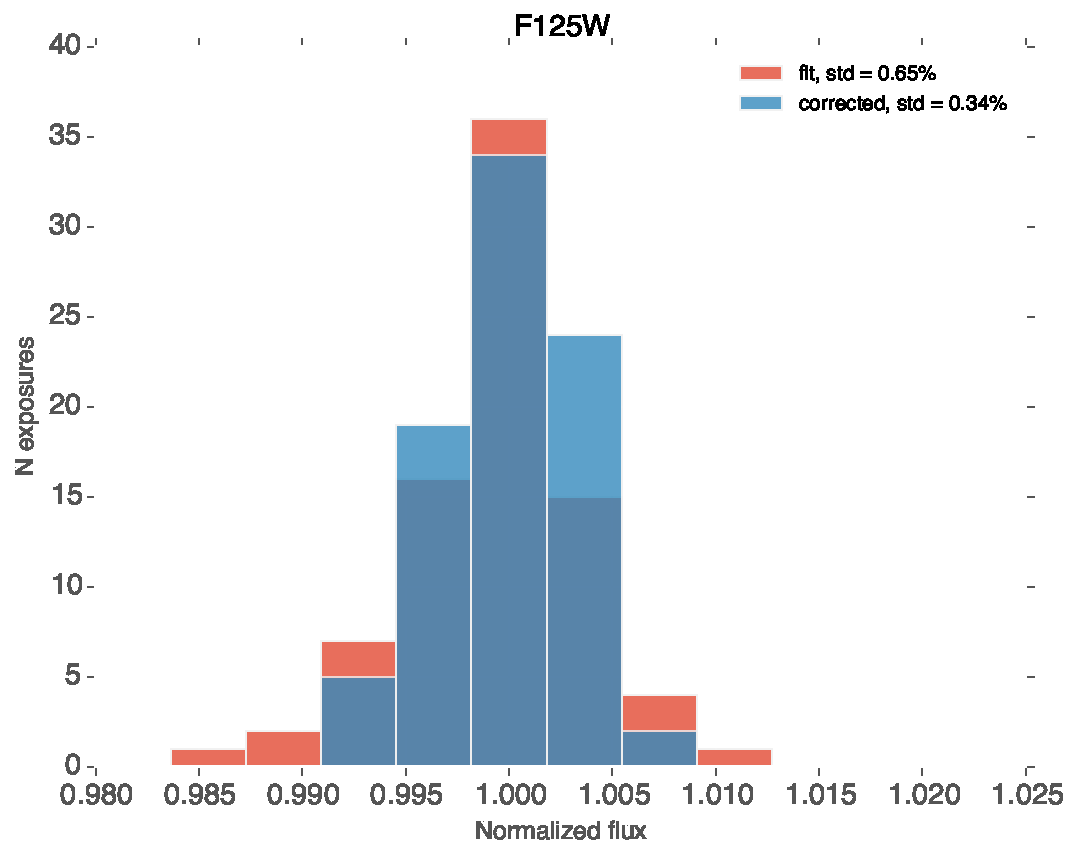
\includegraphics[height=0.9\textheight]{F125W_hist}}
  \only<2>{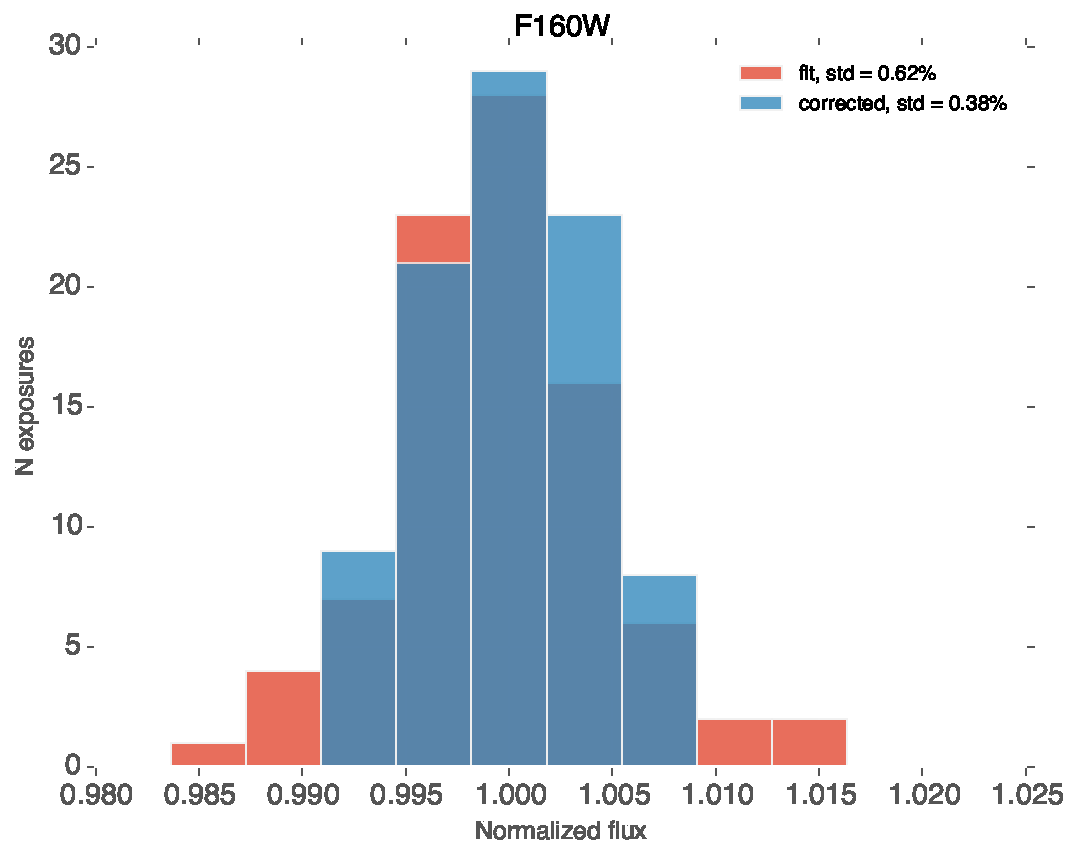
\includegraphics[height=0.9\textheight]{F160W_hist}}
\end{frame}

\begin{frame}
  \frametitle{Light Curve}
  \only<1>{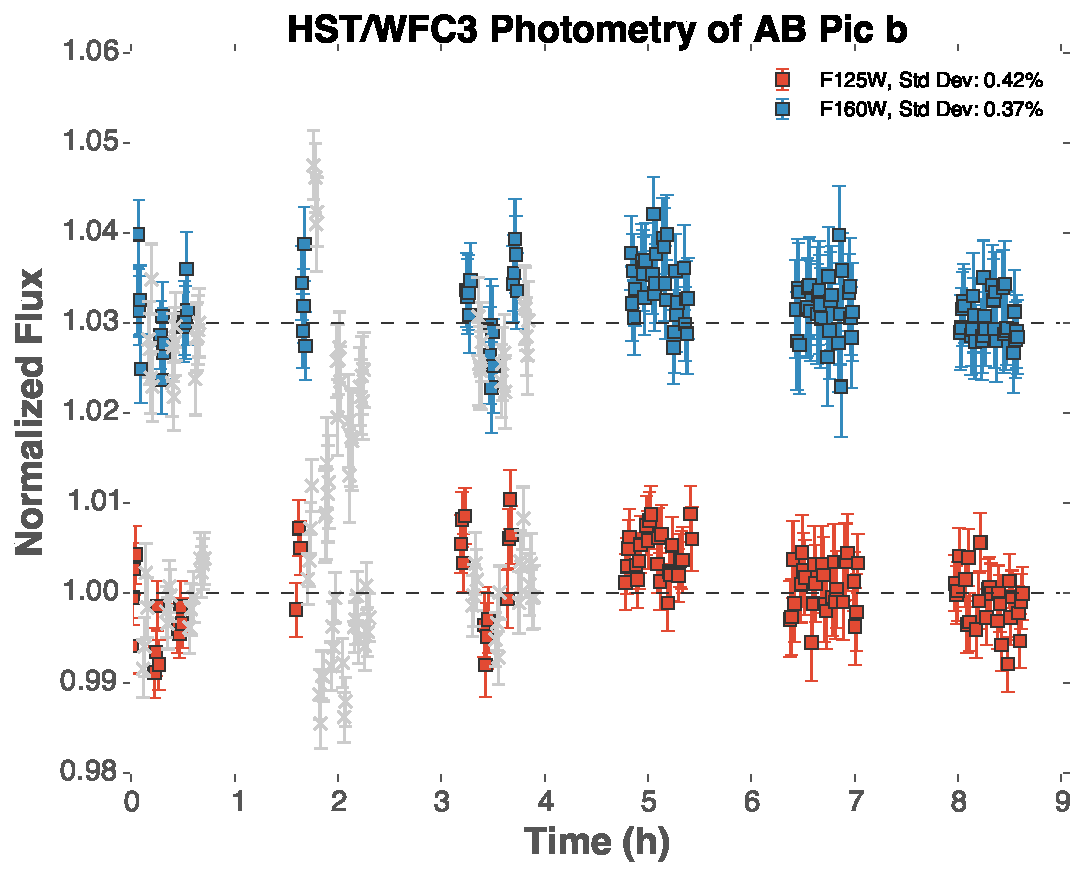
\includegraphics[height=0.9\textheight]{light_curve}}
  \only<2>{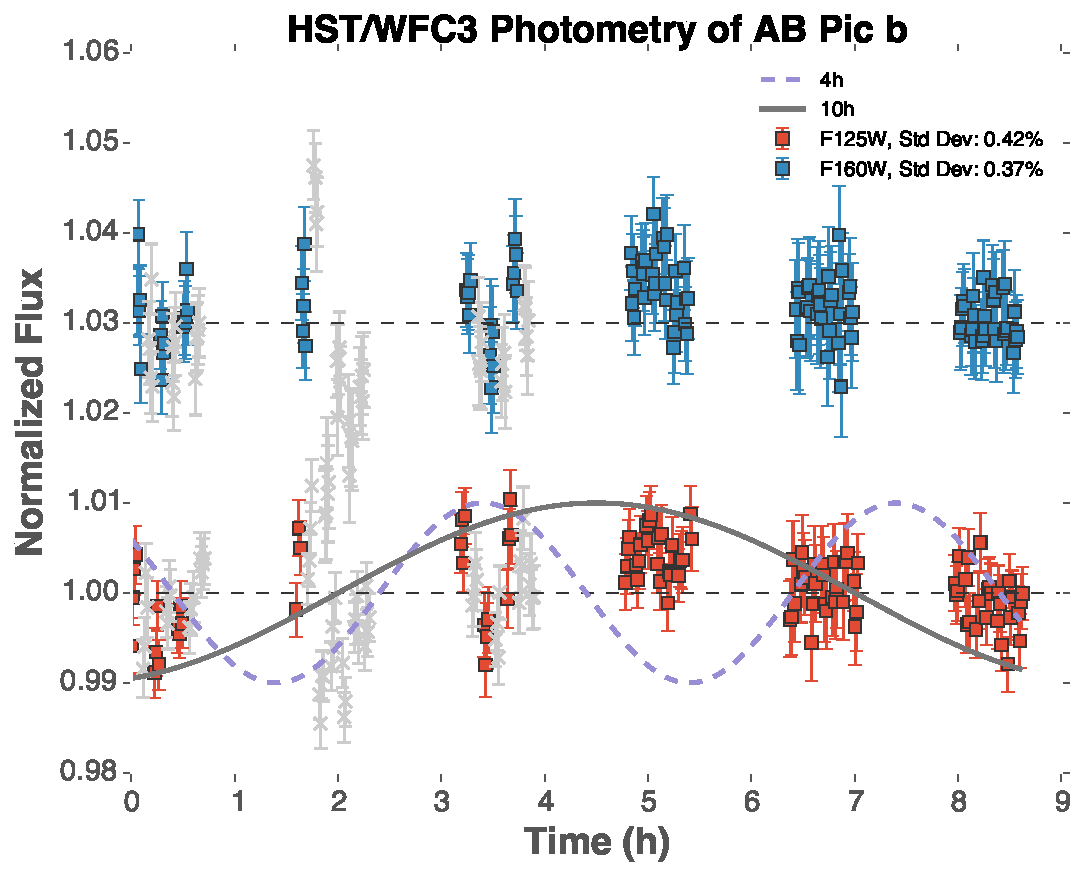
\includegraphics[height=0.9\textheight]{light_curve_with_sin}}
\end{frame}

\begin{frame}
  \frametitle{Status with 2M1207 b}
  \begin{itemize}
  \item Photometry limited by the residual of primary
  \item 3\% precision (5x photon noise)
  \end{itemize}
\end{frame}

\begin{frame}
  \frametitle{Summer plan}
  \begin{itemize}
  \item Finish data reduction with 2M1207 b
  \item Determine a publication strategy
  \item finish one/two paper draft(s)
  \end{itemize}
\end{frame}

\begin{frame}
  \frametitle{Further future plan}
  \only<1>{\structure{HST low mass objects variability survey}\\
    \begin{itemize}
    \item ~20 objects, ~120 orbits
    \item A homogeneous survey that contains low surface gravity, high
      surface gravity objects
    \item spectroscopy and multi-band photometry
    \end{itemize}
  }
  \only<2>{\structure{Brown dwarf atmosphere study with STORM data}\\
    \begin{itemize}
    \item statistical analysis of cloud thickness, variability phase
      shift, etc.
    \end{itemize}
    \structure{Potential side project}
    \begin{itemize}
    \item modeling the patchy clouds
    \end{itemize}
  }
  \only<3>{\structure{Ground based observation}\\
    \begin{itemize}
      \item time resolved spectroscopy
    \end{itemize}
  }
\end{frame}

% \begin{frame}
%   \frametitle{Cloud Keynotes}
%   \only<1>{  \structure{What does cloud mean?}
%   \begin{itemize}
%   \item Solid/Liquid particles formed by condensation
%   \end{itemize}}
% \only<2>{  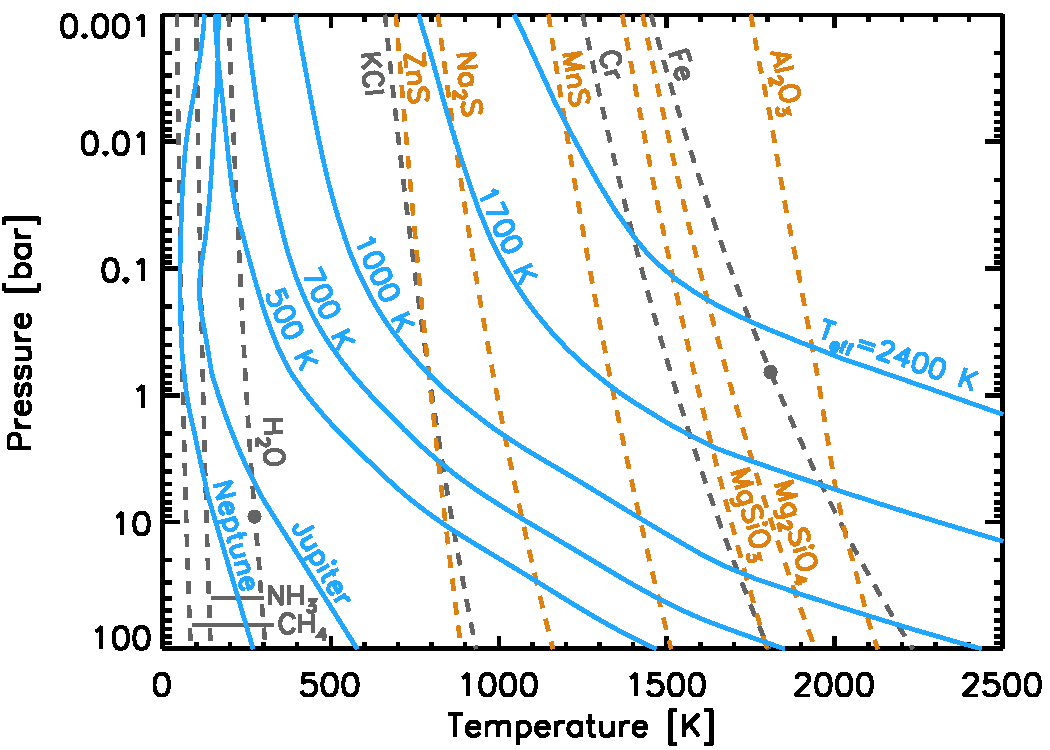
\includegraphics[width=\textwidth]{cond_curves_Fig9}\\
%   \figcite{Marley \& Robinson 2014}}
%   \only<3>{\structure{Scheme of Condensation}
%   \begin{itemize}
%   \item A parcel of gas rises
%   \item Partial pressure exceeds saturation vapor pressure
%   \item Gas condenses, cloud base is determined
%   \item Sentimentation
%   \end{itemize}}
% \only<4>{\structure{Cloud Opacity}
% { \footnotesize \[
%     \tau_\lambda = 75 \epsilon Q^{\rm ext}_{\lambda}(r_{\rm c}) \varphi \biggl({P_{\rm c}\over {1~\rm bar}}\biggr) \biggl({{10^5~\rm cm\,s^{-2}}\over g}\biggr)\biggl({{1~\rm \mu m}\over r_{\rm c}}\biggr)\biggl({{1~\rm g\,cm^{-3}}\over \rho_{\rm c}}\biggr) \
%   \]}
% {\normalsize $r_{\rm c}$ -- particle size\\
% $Q^{\rm ext}_{\lambda}(r_{\rm c})$ -- extinction efficiency\\}
% \figcite{Marley \& Robinson (2014)}}
% \only<5>{\structure{Difficulties}
%   \begin{itemize}
%     \item Chemical equilibrium and condensation are entangled with
%       each other
%     \item Model the phase transition is difficult
%       \item to calculate cloud opacity
%   \end{itemize}
% }
% \end{frame}


% \begin{frame}
%   \frametitle{Model Approaches}
%   \only<1>{
%     \structure{Tsuji Model}
%     \begin{itemize}
%     \item Precipitation described by critical temperature
%       $T_{\mathrm{cr}}$
%       \item Cloud thickness varies with  $T_{\mathrm{cr}}$
%     \end{itemize}
%   }
%   \only<2>{
%     \structure{Allard settl model}
%     \begin{itemize}
%     \item mixing, condensate, coagulation, and sedimentation time
%       scales are bonded by particle size and condensate fraction
%     \item particle size and condensate fraction are calculated to
%       balance those time scales
%     \end{itemize}
%   }
%   \only<3>{
%     \structure{Ackerman \& Marley}
%     \begin{itemize}
%     \item using a scaling factor to describe the relationship of
%       sedimentation velocity and turbulent mixing
%     \item prescribing a particle size distribution 
%     \end{itemize}
%   }
%   \only<4>{
%     \structure{Helling \& Woitke}
%     \begin{itemize}
%     \item Condensation starts with formation of seed particles
%     \item seeds growing by gas-solid surface reaction
%     \end{itemize}
%   }
% \end{frame}

% \begin{frame}
%   \frametitle{Comparison}
%   \begin{columnsonlytextwidth}
%     \begin{column}{0.35\textwidth}
%       \centering
%       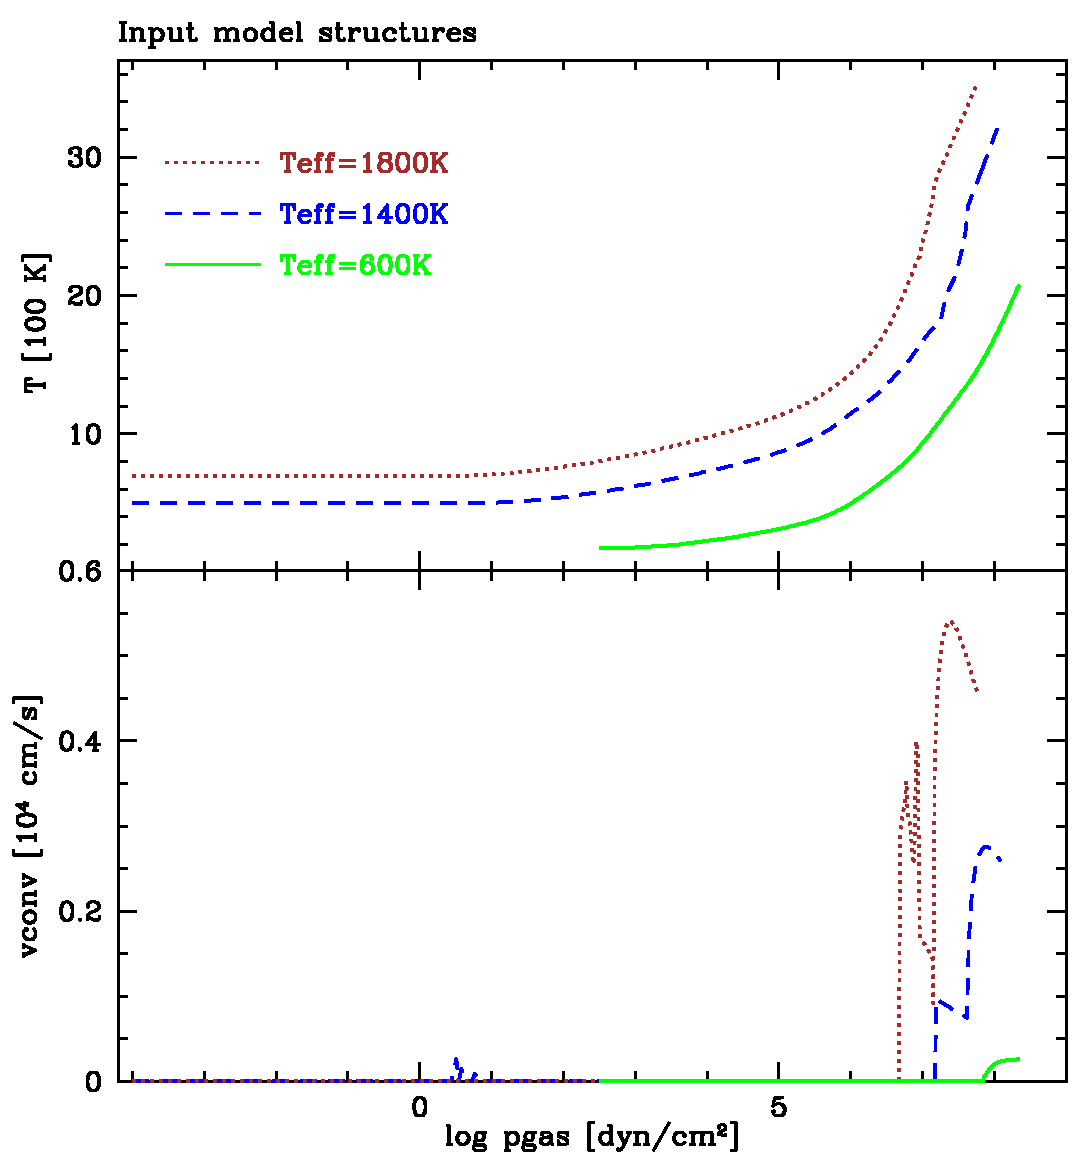
\includegraphics[width=\columnwidth]{InputStructure}
%     \end{column}
%     \begin{column}{0.6\textwidth}
%       \centering
%       \only<1>{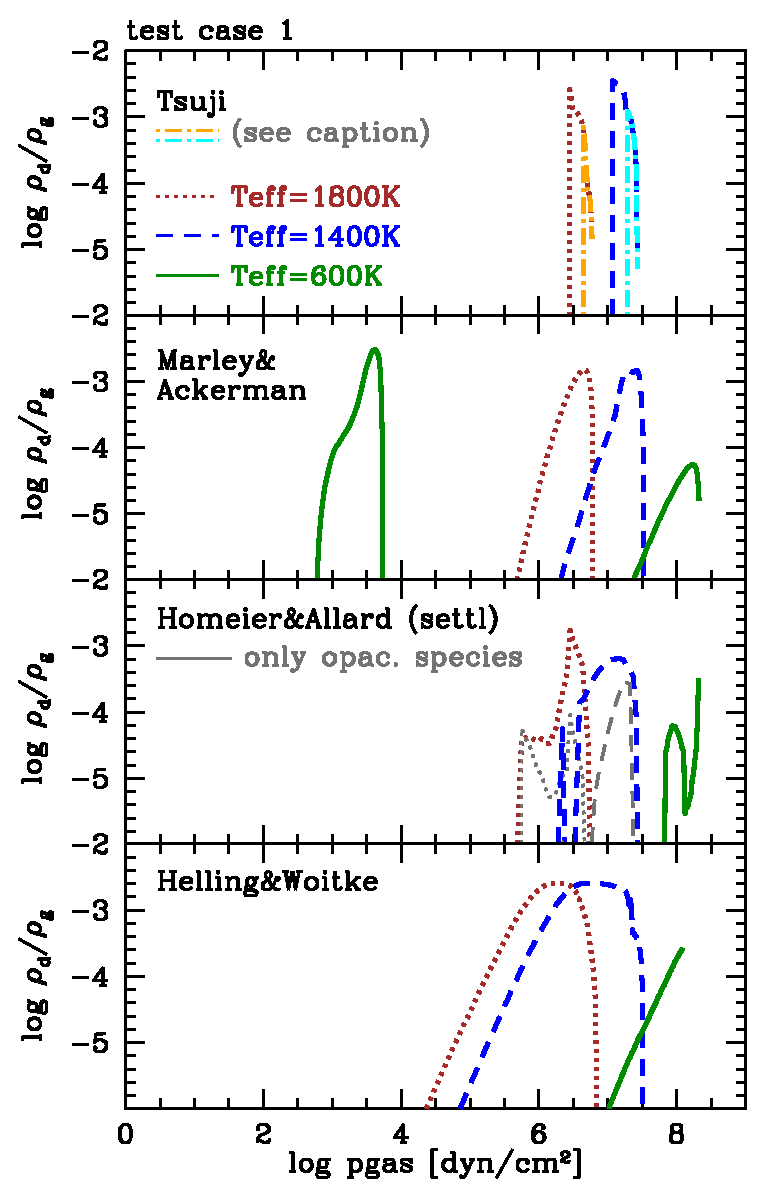
\includegraphics[height=0.8\textheight]{RhodRhoG}}
%       \only<2>{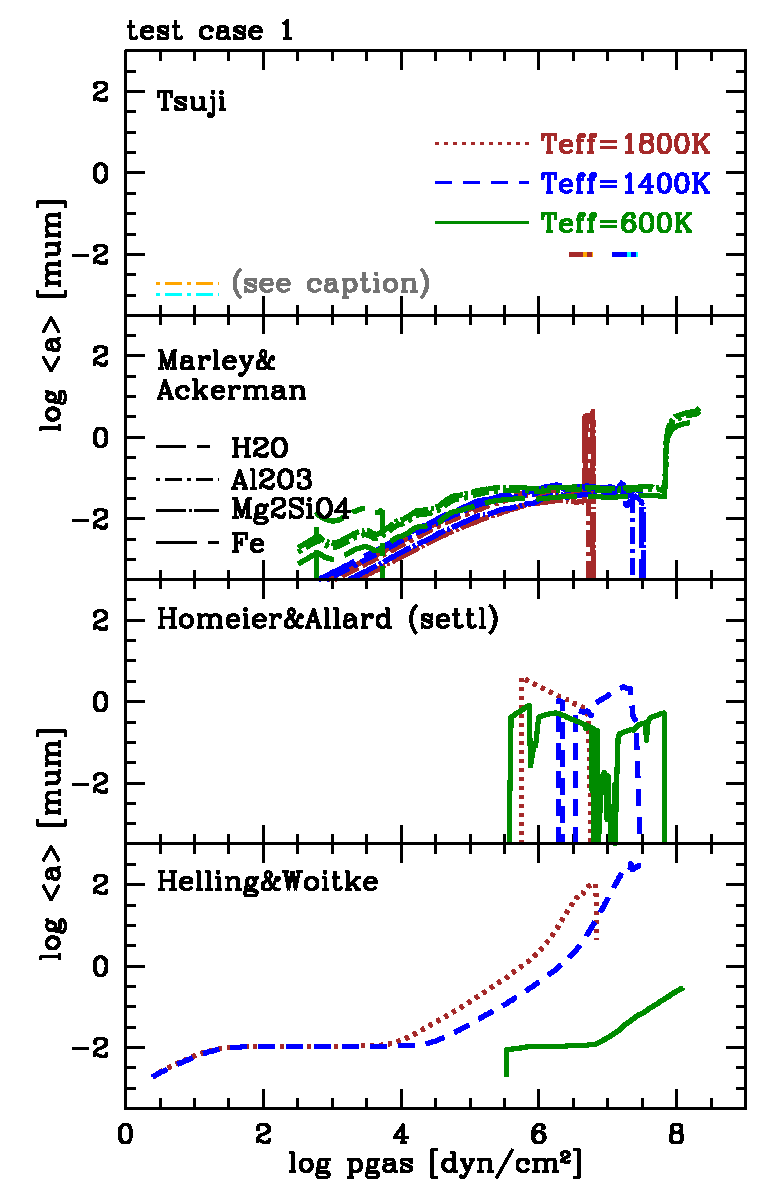
\includegraphics[height=0.8\textheight]{AmeanTC1}}
%     \end{column}
%   \end{columnsonlytextwidth}
%   \figcite{Helling et. al. (2008)}
% \end{frame}

% \begin{frame}
%   \frametitle{Spectrum}
%   \centering
%   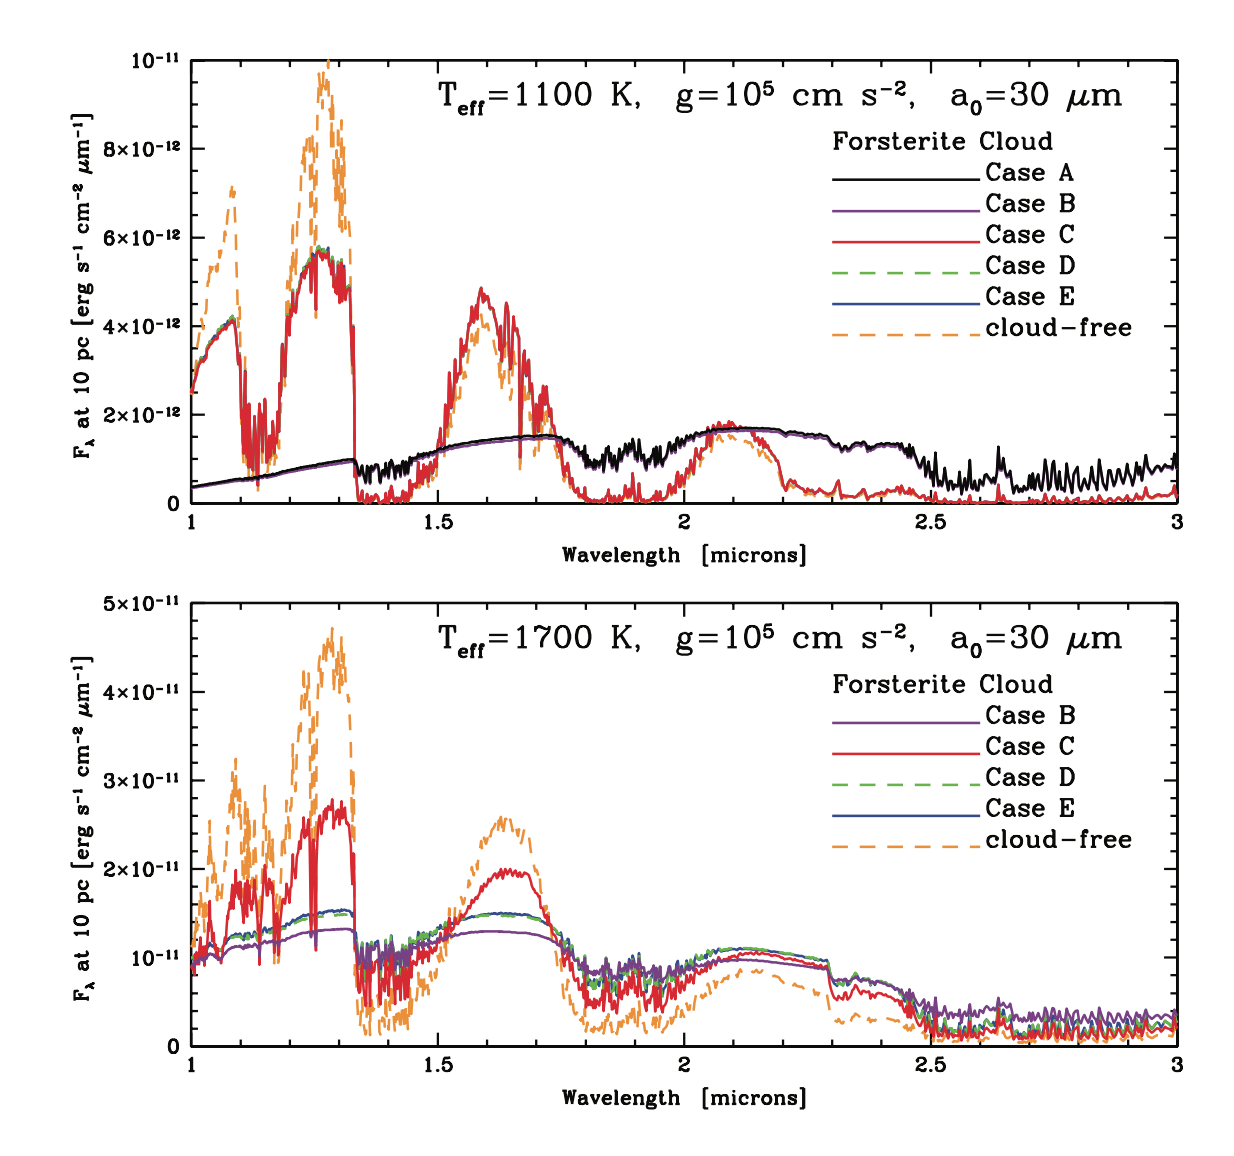
\includegraphics[height=0.85\textheight]{spec}\\
%   \figcite{Burrows et. al. (2006)}
% \end{frame}

% \begin{frame}
%   \frametitle{Patchy Cloud}
%   \begin{itemize}
%   \item Variability of brown dwarfs
%   \item under-luminosity of direct imaged exoplanets and brown dwarfs.
%   \end{itemize}
% \end{frame}

% \begin{frame}
%   \frametitle{Time resolved observation}
%   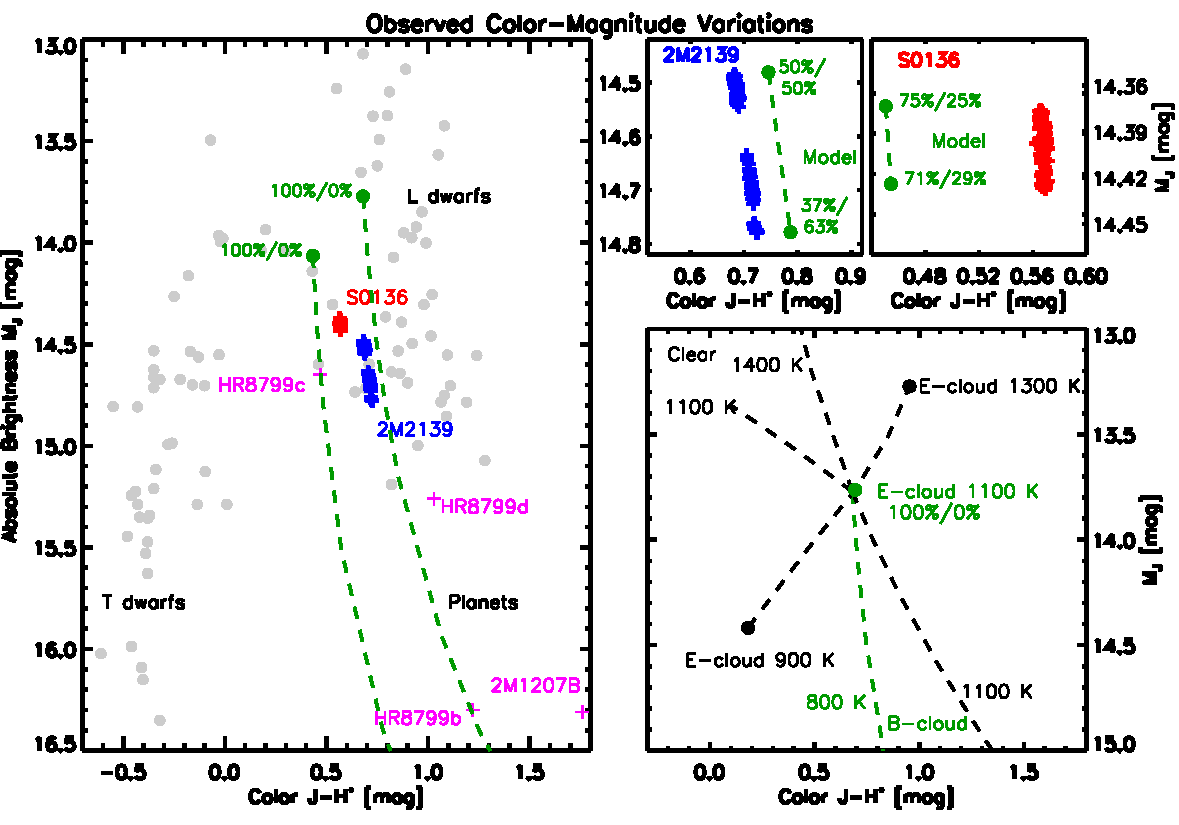
\includegraphics[width=\textwidth]{CMD}\\
%   \figcite{Apai et. al. (2013)}
% \end{frame}

% \begin{frame}
%   \frametitle{Test}

  
% \end{frame}


\end{document}


%%% Local Variables:
%%% mode: latex
%%% TeX-master: t
%%% End:
